\section{Requisiti di sistema}
\subsection{Browser Supportati}

Di seguito viene fornito un breve elenco delle versioni minime dei browser sui quali il funzionamento del nostro plugin è garantito:
\begin{itemize}
	
	\item \gl{Google Chrome} v.55
	\item \gl{Mozilla Firefox} v.50
	\item \gl{Safari} v.10
	\item \gl{Internet Explorer} v.11
	
\end{itemize}

Per un corretto funzionamento del plugin è necessario che sia abilitato \gl{Javascript}.




\section{Configurazione ambiente di lavoro}
\label{sec:configurazione}
\subsection{Installazione di Kibana}
Per poter installare correttamente il prodotto è necessario scaricare e configurare antecedentemente Kibana, reperibile dal link \gl{URL} \url{https://github.com/elastic/kibana/releases}.\\
I plugin sono stati sviluppati con la versione 6.2.2 che si raccomanda anche per l'utilizzo.\\
Una volta scaricato l'archivio compresso sarà necessario estrarre il contenuto in una cartella con nome \texttt{kibana} da raggiungere tramite l'utilizzo di un terminale.
Prima di procedere alla configurazione di Kibana deve essere installato il \gl{framework} \gl{Node.js} ed il relativo gestore di pacchetti chiamato Node \gl{package} manager (npm).\\
Dalla directory corrente, dare il comando \texttt{npm install} per procedere all'installazione dei pacchetti necessari al funzionamento di Kibana.\\
Una volta terminata la configurazione, spostarsi tramite terminale nella cartella \texttt{kibana/bin} ed avviare l'eseguibile \texttt{kibana}.\\
Dopo l'avvio, aprire una finestra di browser e navigare all'indirizzo URL \url{localhost:5601} per raggiungere la \gl{dashboard} di Kibana.
\subsection{Installazione dei plugin per lo sviluppo}
Per prima cosa bisogna provvedere a scaricare i plugin. Questi si possono scaricare da \href{https://github.com/SWEeftyTeam/Havana}{https://github.com/SWEeftyTeam/Havana} cliccando sul pulsante verde "Clone or download" e poi su "Download ZIP".
Per l'installazione, estrarre dall'archivio compresso le cartelle dei plugin come illustrato in figura:
\begin{figure}[H]
	\centering 
	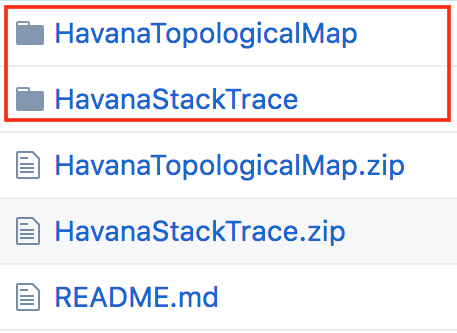
\includegraphics{Images/strutturadev}
	\caption{Files da utilizzare per l'installazione finalizzata allo sviluppo}
\end{figure}
Spostare le cartelle dei plugin nella stessa \gl{directory} in cui si trova la cartella \texttt{kibana}, ottenendo la seguente struttura finale.\\
\begin{figure}[H]
	\centering 
	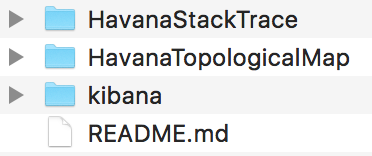
\includegraphics{Images/pos}
	\caption{Struttura delle cartelle in relazione a Kibana}
\end{figure}
Aprire una finestra di terminale, navigare all'interno della cartella del plugin di cui si vuole effettuare lo sviluppo e utilizzare il comando \texttt{npm install} per avviare l'installazione dei moduli node necessari al funzionamento del plugin.
Una volta completata l'installazione, per avviare Kibana in modalità sviluppo con il plugin desiderato dare il comando \texttt{npm start} dalla directory corrente.

\subsection{Installazione dei plugin per l'utente finale}
Per prima cosa bisogna provvedere a scaricare i plugin. Questi si possono scaricare da \href{https://github.com/SWEeftyTeam/Havana}{https://github.com/SWEeftyTeam/Havana} cliccando sul pulsante verde "Clone or download" e poi su "Download ZIP".
Per l'installazione dei plugin in una \gl{directory} a scelta utilizzare il comando \texttt{install} con l'opzione \texttt{-d} o \texttt{--plugin-dir}  specificando una directory per i plugin, come nell'esempio seguente:
\begin{lstlisting}
$ bin /kibana-plugin install \gl{file}:///some/local/path/my-plugin.zip -d path/to/directory 
\end{lstlisting}
Una volta completata l'installazione è possibile navigare tra tutti i plugin installati nella lista presente nel menù a sinistra di Kibana.
\begin{figure}[H]
	\centering 
	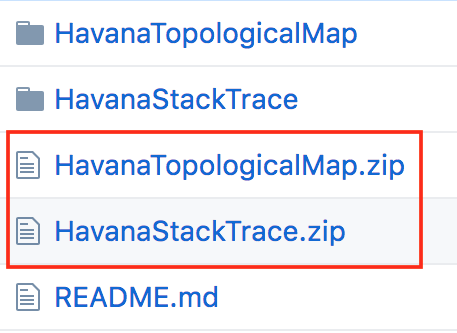
\includegraphics{Images/strutturauser}
	\caption{Files da utilizzare per l'installazione finalizzata all'utente finale}
\end{figure}
\subsection{Configurazione di Elasticsearch}
Kibana si appoggia ad Elasticsearch per prelevare i dati da monitorare, quindi sarà necessaria un'istanza di esso che si può avere in locale o remoto configurando il file \texttt{kibana.yml} all'interno della cartella \texttt{config}, in particolare il campo \texttt{elasticsearch.url: "localhost:9200"} che dovrà essere modificato con l'indirizzo dove risiede l'istanza remota di Elasticsearch.\\
Localmente invece, scaricare il pacchetto dal link URL \url{https://www.elastic.co/downloads/elasticsearch}, versione raccomandata 6.2.2.
Una volta scaricato l'archivio compresso, estrarre il contenuto in una cartella locale, raggiungerla tramite terminale ed entrare nella sottocartella \texttt{bin} da dove avviare l'eseguibile \texttt{elasticsearch}.\\
L'istanza sarà interrogabile all'indirizzo URL \url{localhost:9200}.

\section{Estendibilità}
\subsection{Modifica delle funzionalità presenti}
\subsubsection{Mappa topologica}
\label{sec:graph}
Per poter cambiare gli aspetti di visualizzazione della mappa topologica è necessario modificare il file \texttt{d3functions.js} presente nella cartella \texttt{public/d3utilities} ove è possibile trovare le seguenti variabili usate dalla libreria \gl{D3.js} per comporre gli elementi del grafo:
\begin{itemize}
	\item \texttt{svg}: Canvas del grafo;
	\item \texttt{color}: Schema colori;
	\item \texttt{simulation}: Gestore per i comportamenti fisici del grafo;
	\item \texttt{link}: Archi tra componenti;
	\item \texttt{linkLabel}: Etichette degli archi rappresentanti i tempi medi;
	\item \texttt{connectionLabel}: Etichette degli archi rappresentanti il tipo di richiesta effettuata;
	\item \texttt{node}: Nodi del grafo rappresentanti i componenti monitorati;
	\item \texttt{nodelabels}: Etichette con il nome identificativo dei nodi.
\end{itemize}
Ad esempio modificando l'attributo \texttt{style} della variabile \texttt{link} si possono aggiungere ulteriori colorazioni condizionate per gli archi tra i componenti, mentre editando l'attributo \texttt{xlink:href} della variabile \texttt{node} si possono introdurre nuove icone per nuovi componenti monitorati. \\
Per immettere ulteriori icone, copiare i file \texttt{.svg} nella directory dedicata \texttt{public/res/img} ed importarle poi con il seguente codice:
\begin{lstlisting}
import exampleSvg from "plugins/plugin-havana/res/img/example.svg";
\end{lstlisting}
nel file \texttt{d3functions.js}.\\
Inoltre nel costruttore della classe \texttt{D3Helper} è presente la soglia limite denominata \texttt{timeLimit}, oltre alla quale gli archi colleganti i nodi della mappa interessati verranno colorati in rosso per mettere in risalto eventuali errori o tempi di risposta tra componenti eccessivamente lunghi.
Si è prestabilito un valore di ritorno pari a 3000ms che può essere modificato a seconda delle necessità anche introducendo algoritmi per un calcolo dinamico della soglia limite. \\
Infine sono disponibili le funzioni per la gestione di azioni come zoom, drag e click per i vari componenti della mappa:
\begin{itemize}
	\item \texttt{zoomed()}: applica il metodo \texttt{d3.event.transform};
	\item \texttt{ticked()}: posiziona ogni oggetto alle coordinate x ed y nel canvas;
	\item \texttt{dragged()}: sposta alle coordinate \texttt{d3.event.x} e \texttt{d3.event.y} l'oggetto coinvolto nel trascinamento;
	\item \texttt{dragstarted()}: attiva l'elemento da trascinare.
\end{itemize}
Modificando ad esempio l'attributo x ed y di \texttt{nodelabels} all'interno della funzione \texttt{ticked} è possibile spostare il posizionamento dell'etichetta rappresentante l'identificativo del nodo rispetto all'icona del nodo stesso.\\

\subsubsection{Stack trace}
\label{sec:stack}
Per poter cambiare gli aspetti di visualizzazione della stack trace è necessario modificare il file \texttt{index.\gl{HTML}} presente nella cartella \texttt{plugin/templates}.\\
Oltre alle modifiche apportabili al codice HTML e \gl{CSS}, è possibile cambiare il comportamento di alcune funzioni Javascript che regolano l'espansione e la compressione di una riga della stack trace o lo switch tra la visualizzazione di un call tree e le query ad esso associate.\\
Attraverso delle direttive \gl{AngularJS} è possibile sfruttare in maniera ottimale i dati provenienti da \$scope.nodes che rappresenta un array contenente tutte le trace di nostro interesse.\\
Inoltre nel file \texttt{app.js} presente nella cartella \texttt{plugin} sono state implementate delle direttive personalizzate AngularJs per la gestione del call tree di ogni trace, che sono:
\begin{lstlisting}
.directive("tree", function() {..})
\end{lstlisting}
e
\begin{lstlisting}
.directive("branch", function($compile) {...})
\end{lstlisting}
Queste due direttive funzionano in modo innestabile tra loro permettendo di visualizzare i vari metodi appartenenti ad un call tree seguendo la struttura gerarchica con cui sono stati salvati nella variabile \$scope.nodes.calltree.

\subsection{Architettura dei plugin Kibana}
\label{sec:architettura}
Ogni plugin per Kibana è articolato in due sezioni principali: lato client e lato server. Il lato client viene eseguito sul browser dell'utente che utilizza il plugin, mentre il lato server sul server di Kibana all'interno del quale esso è installato. Il lato client deve fare richieste al lato server per ottenere i dati di Elasticsearch, mentre il lato server deve rispondere ad esse interrogando un'istanza del database. Si presenta di seguito la forma che hanno i dati sul database Elasticsearch e il dettaglio delle due componenti del sistema.

\paragraph{ElasticsearchClient} \Spazio
\texttt{ElasticsearchClient} è il componente che si occupa di eseguire le chiamate API al lato server. Non è una classe vera e propria all'interno del codice, ma un \emph{Service}. 
I Service sono funzioni, od oggetti, che possono essere passati a tutte le altri componenti di AngularJS attraverso \emph{Dependency Injection}, permettono di condividere codice e funzionalità facilmente. Essi sono \emph{lazily instantiated}, cioè generati solo quando un componente esprime una dipendenza verso un determinato service. Permettono la realizzazione di servizi come i client API, dove avere piú istanze dello stesso client non sarebbe ragionevole. 
Utilizzare un service è l'unico modo per poter eseguire chiamate REST parametrizzate al lato server. Ciascun metodo qui presentato nasconde in realtà una chiamata GET all'opportuno componente lato server. 
Il tipo di ritorno dei \texttt{Services} è una \texttt{Promise} di un qualche altro tipo. Questo significa che la risposta \emph{non è sincrona}, ovvero bisgnerà attendere che il lato server risponda per utilizzare la \texttt{Promise}. Ciò viene fatto utilizzando il metodo \texttt{then} sulla \texttt{Promise}. Nel blocco del metodo dovrà essere specificato il comportamento da eseguire sulla risposta della \texttt{Promise} eseguita. Per una descrizione più dettagliata si rimanda alla documentazione di Mozzilla: \href{https://developer.mozilla.org/en-US/docs/Web/JavaScript/Reference/Global\_Objects/Promise}{https://developer.mozilla.org/en-US/docs/Web/JavaScript/Reference/Global\_Objects/Promise} .

I metodi esposti da \texttt{ElasticsearchClient} sono: 
\begin{itemize} 
	\item \texttt{tracesIndices(): Promise<Array<String>>} ritorna un array di stringhe che rappresenta gli indici contenuti nell'istanza di ElasticSearch che hanno all'interno delle traces, ovvero i dati utili al plugin; 
	\item \texttt{getIndex(index:String): Promise<ElasticsearchIndexResult>} ritorna al chiamante i dati grezzi che vengono restituiti da Elasticsearch eseguendo una ricerca priva di parametri sull'indice passato come parametro, ovvero \texttt{index}. Essi comprendono, oltre tutti i documenti dell'indice, anche i metadati di Elasticsearch dato che sono di tipo \texttt{ElasticsearchIndexResult}. È anche possibile specificare un numero massimo di documenti ritornati al chiamante o una particolare tipologia letta nel database di tipo \texttt{server} o \texttt{database}; 
	\item \texttt{getData(indices:Array<String>): Promise<Array<ElasticsearchIndexResult>>}: ritorna al chiamante un array di dati grezzi, ognuno dei quali rappresenta il risultato di una ricerca priva di parametri su un indice. Gli indici letti sono quelli ritornati da \texttt{tracesIndices()}, ovvero tutti e soli quelli che contengono traces. 
\end{itemize} 

\paragraph{DataReader} \Spazio
\label{sec:DataReader}
\texttt{DataReader} è il componente del sistema che si occupa di reperire i dati da Elasticsearch, ciò viene fatto utilizzando il \emph{Service} \texttt{ElasticsearchClient}. Sarebbe effettivamente possibile utilizzare le chiamate al \emph{Service} ogni qualvolta fossero necessari dei dati, tuttavia ricordiamo che tali chiamate non vengono racchiuse all'interno di un oggetto ben strutturato. DataReader restituirà ai richiedenti le informazioni grezze i tipo \texttt{ElasticsearchIndexResult}, esattamente come vengono restituite da Elasticsearch. Anche \texttt{DataReader} restituisce \texttt{Promise} come \texttt{ElasticsearchClient}.

I metodi di \texttt{DataReader} sono:  

\begin{itemize} 
	\item \texttt{constructor(esClient:ElasticsearchClient): void} che costruisce il \texttt{DataReader} parametrizzato con un \texttt{ElasticsearchClient};
	\item \texttt{setElasticsearchClient(esClient:ElasticsearchClient): void}: permette di impostare una sorgente dei dati;
	\item \texttt{tracesIndices(): Promise<Array<String>>}: ritorna un array di stringhe, i quali elementi sono tutti e soli gli indici all'interno dell'istanza di Elasticsearch che hanno al loro interno delle traces;
	\item \texttt{readIndex(index:String): Promise<ElasticsearchIndexResult>}: ritorna al chiamante i dati grezzi che vengono restituiti da Elasticsearch eseguendo una ricerca priva di parametri sull'indice passato come parametro, ovvero \texttt{index}. Essi comprendono oltre tutti i documenti dell'indice anche i dati amministrativi di Elasticsearch;
	\item \texttt{readData(): Promise<Array<ElasticsearchIndexResult>>}: ritorna al chiamante un array di dati grezzi, ognuno dei quali rappresenta il risultato di una ricerca priva di parametri su un indice. Gli indici letti sono quelli contententi delle traces, ovvero quelli utili al plugin. Ciò è realizzato leggendo tali indici grazie al metodo \texttt{tracesIndices()}.
\end{itemize}

\paragraph{DataCleaner}\Spazio
\label{sec:DataCleaner}
\texttt{DataCleaner} è il componente del sistema che si occupa di pulire i dati grezzi che sono stati reperiti da Elasticsearch. Esso compie questo lavoro in due momenti: prima estraendo i dati utili (ovvero i documenti veri e propri) da Elasticsearch e poi pulendoli attraverso una \emph{strategy}.\\
I suoi metodi sono:

\begin{itemize} 
	\item  \texttt{constructor(strategy:CleanerStrategy): void} costruisce il \texttt{DataCleaner} con una specifica strategia di pulizia;
	\item \texttt{setStrategy(in strategy:CleanerStrategy): void} il quale riceve in input un oggetto che implementa l'interfaccia \texttt{CleanerStrategy} e lo assegna al riferimento proprio dell'oggetto;
	
	\item \texttt{cleanData(in elasticsearchIndicesResults:Array<ElasticsearchIndexResult>): Array<Request>} il quale prima rimuove i metadati (chiamando il suo metodo \\ \texttt{ removeMetaDataFromIndices }) di Elasticsearch dal parametro in input e successivamente chiama l'implementazione di \texttt{clean} della strategia che possiede al suo interno.  Tale strategia è incaricata di raffinare ulteriormente i dati per la costruzione della Mappa Topologica oppure per la costruzione dello Stack Trace tramite il metodo \texttt{clean};
	
	\item \texttt{removeMetadataFromIndices(elasticsearchIndicesResults: \\Array<ElasticsearchIndexResult>): Array<Request>}  si occupa di rimuovere i metadati di Elasticsearch da un Array di indici invocando il metodo\\ \texttt{removeMetaDataFromIndex} su ognuno dei singoli indici. Viene ritornato un array di \texttt{Request} che rappresenta le traces lette dai vari indici in un singolo array;
	
	\item \texttt{removeMetadataFromIndex(elasticsearchIndexResult:ElasticsearchIndexResult): Array<Request>} il quale si occupa di rimuovere i metadati di Elasticsearch che sono presenti in un \emph{singolo} indice. Questo metodo ritorna un array contenente i documenti \gl{JSON} così come essi sono stati inseriti dall'applicazione di monitoring negli indici di Elasticsearch. Elasticsearch, infatti, immagazzina i documenti JSON nel campo \texttt{\_source} il quale è inserito in oggetti che contengono altri dati ed informazioni amministrative. Il metodo si occupa di rimuovere questi dati e restituire un array contenente i documenti di un indice.
\end{itemize}


\subsection{Sviluppo di nuove funzionalità}
\label{sec:nuovefunzionalita}
Per poter sviluppare nuove modalità di visualizzazione dei dati è possibile avvalersi delle classi \texttt{DataReader} e \texttt{DataCleaner} già presenti all'interno della cartella \texttt{public/components} dei plugin, creando quindi in questa directory una classe \texttt{Builder} per strutturare le informazioni da passare al \gl{frontend} dell'applicazione secondo una nuova strategia da creare nella sottocartella \texttt{strategies}.\\
Lo sviluppo del frontend può essere eseguito modificando adeguadatamente alle esigenze i file:
\begin{itemize}
	\item \texttt{app.js} presente nella cartella \texttt{public} dei plugin;
	\item \texttt{d3functions.js} presente nella cartella \texttt{public/d3utilities} del plugin relativo alla mappa topologica;
	\item \texttt{index.html} presente nella cartella \texttt{public/templates} dei plugin.
\end{itemize}
Nel primo file sarà necessario importare la classe \texttt{Builder} e la relativa strategia prodotta:
\begin{lstlisting}
let ExampleBuilder = require("./components/exampleBuilder");
let ExampleCleaner = require("./components/strategies/examplecleaner");
\end{lstlisting}
per poter poi istanziare i relativi oggetti necessari allo sviluppo del frontend.



\newpage
\appendix
\section{Glossario}

\lettera{A}

\parola{AngularJS}{Framework front-end open-source scritto in Javascript, creato e manutenuto da Google. È di tipo MVC (Model View Controller) nato per sopperrire alle difficoltà che si incontrano quando si sviluppano web app.}

\parola{Architettura}{Organizzazione fondamentale di un sistema, definita dai suoi componenti, dalle relazioni reciproche tra i componenti e con l'ambiente, e i principi che ne governano la progettazione e l'evoluzione.}

\lettera{B}

\parola{Backend}{Parte dell'architettura non visibile dall'utente, generalmente si occupa di elaborare i dati ricevuti in input dall'utente. }

\lettera{C}

\parola{Call tree}{Albero delle chiamate, rappresenta l'insieme delle chiamate a funzioni o funzionalità del sistema eseguite da un programma.}

\parola{CSS}{Linguaggio usato per definire la formattazione di documenti HTML, XHTML e XML ad esempio i siti web e relative pagine web.}

\lettera{D}

\parola{Database}{Archivio di dati strutturato in modo da razionalizzare la gestione e l'aggiornamento delle informazioni e da permettere lo svolgimento di ricerche complesse.}

\parola{Directory}{Entità del file system che elenca altre entità, tipicamente file e altre directory, e che permette di organizzarle in una struttura ad albero.}

\parola{D3.js}{Libreria JavaScript per creare visualizzazioni dinamiche ed interattive, partendo dati organizzati, visibili attraverso un comune browser.}

\lettera{E}

\parola{Elasticsearch}{Motore di ricerca open-source. Dispone di API molto estensive ed elaborate. Può effettuare ricerche in maniera molto performante.}

\lettera{F}
\parola{Framework}{Architettura logica di supporto (spesso un’implementazione logica di un particolare design pattern) su cui un software può essere costruito per facilitarne lo sviluppo da parte del programmatore.}

\parola{Frontend}{Parte di un software che un utente può vedere e con il quale può interagire.}

\lettera{G}
\parola{GitHub}{Servizio web di hosting per progetti software che utilizzano Git come sistema di versionamento.}
\parola{Google Chrome}{Google Chrome è un browser web sviluppato da Google, basato sul motore di rendering Blink.}


\lettera{H}
\parola {Hardware}{Insieme delle componenti fisiche, non modificabili, di un sistema di elaborazione dati.}

\parola{HTML (Hypertext Markup Language)}{Linguaggio standardizzato per la definizione della struttura logica di una pagina web.}

\lettera{I}
\parola{Internet Explorer}{Browser web grafico proprietario sviluppato da Microsoft e incluso in Microsoft Windows a partire dal 1995.}
\parola{Issues}{Sistema di gestione di problemi di un progetto su Github.}

\lettera{J}

\parola{JavaScript}{Linguaggio di scripting utilizzato principalmente per applicazioni web.}

\parola{JSON (JavaScript Object Notation)}{Formato di file standard che utilizza un testo comprensibile dall'uomo per trasmettere dati costituiti da coppie valore-attributo.}

\lettera{K}

\parola{Kibana}{Framework open source per la visualizzazione dei dati salvati su Elasticsearch.}

\lettera{M}

\parola{Mappa topologica}{Visualizzazione sotto forma di grafo dei componenti di un'applicazione in cui i componenti come server e database sono i nodi e le interazioni fra essi, ovvero le richieste fatte da un componente ad un altro (come richieste HTTP o queries), sono gli archi.}

\parola{Mozilla Firefox}{Web browser libero e multipiattaforma, mantenuto da Mozilla Foundation.}

\lettera{N}
\parola{Node.js}{Runtime Javascript costruito sul motore JavaScript V8 di Chrome. Molti dei suoi moduli base sono scritti in Javascript, e gli sviluppatori possono scrivere nuovi moduli in Javascript. }  

\lettera{P}
\parola{Plugin}{Programma non autonomo che interagisce con un altro programma per ampliare o estendere le funzionalità originarie.}  

\parola{Prodotto}{Indica il risultato di un'attività, sia esso un documento, del codice sorgente o un qualsiasi risultato verificabile che possa essere offerto per soddisfare un bisogno o un’esigenza.}  

\parola{Progetto}{Insieme di attività e compiti che prevedono il raggiungimento di determinati obiettivi con specifiche fissate. Sono definite date di inizio e fine durante la quale si può predisporre di limitate risorse che vengono consumate nello svolgersi delle attività. }  

\lettera{R}
\parola{Repository}{Ambiente di un sistema informativi in cui vengono gestiti e depositati documenti e file}

\lettera{S}

\parola{Safari}{Web browser multipiattaforma, sviluppato e mantenuto da Apple.}

\parola{Server}{Componente o sottosistema informatico di elaborazione e gestione del traffico di informazioni che fornisce, a livello logico e fisico, un qualunque tipo di servizio ad altre componenti.}

\parola{Stack Trace}{Lista di un insieme di traces prese in esame.}

\lettera{T}

\parola{Trace}{Struttura dati che rappresenta una singola richiesta effettuata fra due componenti di una applicazione monitorata oppure fra un utente esterno e un componente dell'applicazione. Viene solitamente memorizzata in un database per successiva analisi.}

lettera{U}
\parola{URL}{\emph{Uniforme Resource Locator}, indirizzo simoboli per riferirsi ad una risorsa in rete.}



